\section{The Predecease of Parents, with Examples (30K,31P)}

\textbf{/101K;96P/} Some astrologers have explained the topic of the predecease of parents in one way, others in another
way. We have tested these methods and have found the following. Since the Sun indicates the father (as does Saturn in the second rank), the most accurate <procedure>, for night and day births, is to examine
<which of these two> stars is associated \mn{Associated Planets} with the \Moon, i.e. beheld by the \Moon, in conjunction with the \Moon, or in the <\Moon’s> house or triangle. That star assumes the Father’s Place. \Venus\xspace and the \Moon\xspace assume the Mother’s Place, using the same procedure. 

So for each nativity it will be necessary to determine which star is beheld by malefics or which star is unfavorably situated, whether \Sun, \Moon, \Venus, or \Saturn\xspace (although the latter is already the destroyer of the father). If the \Sun\xspace assumes the Father’s Place and is beheld by \Mars\xspace or \Saturn\xspace with no benefics in aspect, the forecast of predecease will apply to the father. If the same is true of the \Moon\xspace or \Venus, the forecast will apply to the mother. If both the luminaries or \Venus\xspace are beheld by malefics, the star unfavorably situated or in another’s sect will indicate the predecease.

Another method: the Father’s Lot in a masculine sign or its ruler with a malefic in aspect indicates the father’s predecease. Likewise the same thing happens with respect to the Mother’s Lot, especially if one knows for certain that the father is alive.

Another method: determine the number of days from the rising of Sirius to the birth date. Divide this figure by 12 and count the remainder (less than 12) from the \Moon’s position, giving one to each sign. If the count stops at a masculine sign, the father will predecease; if at a feminine sign, the mother will
predecease. For example, take the nativity cited below, Mechir 13: from the rising of Sirius on Epiphi 25 to Mechir 13 are 203 days. Divide this by 12, and the remainder is 11. Count this from the \Moon\xspace in \Scorpio\xspace and stop in \Virgo, a feminine sign. \Mars\xspace is also in that sign. The mother will die first.

An example: \Sun, \Mercury\xspace in \Aquarius, \Moon\xspace in \Scorpio, \Saturn\xspace in \Cancer, \Jupiter\xspace in \Libra, \Venus\xspace in \Capricorn, \Mars, Ascendant in \Virgo
\footnote{\textit{Greek Horoscopes} dates the chart (L120) to approximately February 8, 120AD (p.116)}.

\clearpage
\begin{wrapfigure}[15]{R}{7cm}
\centering
\vspace{-20pt}
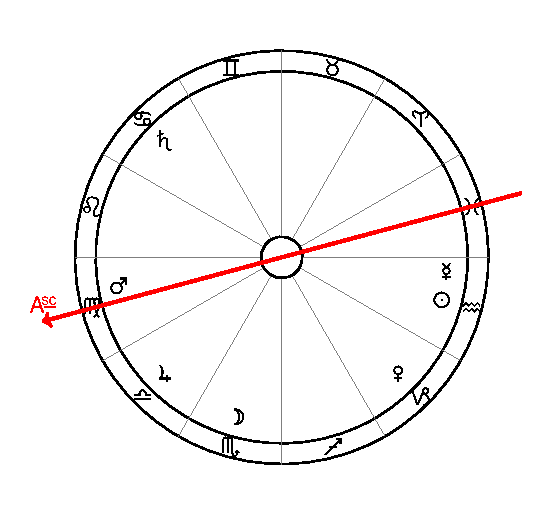
\includegraphics[width=0.68\textwidth]{charts/2_30_1}
\caption{Chart 19 [II.30.1, GH L120]}
\label{fig:chart19}
\end{wrapfigure}

For night births, \Saturn\xspace is associated \textbf{/102K/} with the \Moon\xspace because it is found in \Cancer <same triangle> and is the houseruler of the \Sun\xspace. \Saturn\xspace assumes the Father’s Lot/Place and was beheld by \Jupiter, with \Venus\xspace \textbf{/97P/} in Good Daimon. The \Moon\xspace and \Venus, which are beheld by two malefics, indicated the predecease of the mother.

Another method: if the \Sun\xspace is in superior aspect with the \Moon, the mother will predecease; if the \Moon\xspace is in superior aspect with the \Sun, the father will predecease. If neither of these is superior to the other and if they are unconfigured, I examine \Saturn\xspace and \Venus. If these <are unconfigured>, I examine \Saturn\xspace and the \Moon. 

If the \Sun\xspace is in superior aspect\mn{Aspect Intercept}, but \Venus\xspace is between, \Venus\xspace will intercept the superior aspect
\footnote{Intercepted aspects often appear as a Horary technique.}. Then look to see if \Saturn\xspace is in inferior aspect with \Venus, and if so there will be the premature decease of the father—or the reverse, if \Venus\xspace is inferior to Saturn. 

If \mn{Superior Aspect} the star that intercepts the stars of superior aspect has itself a superior influence, the intercepting stars will have the ability to bring about their own effects. (The superior aspecting happens in the same signs or in those in opposition. In general a star which heads for/aims at another <from the right> is in superior aspect to the other; the same
is true of a star which has a correspondingly <?> superior power.)

\newpage
